\documentclass[10pt,a4paper,dvipdfmx,uplatex]{jsarticle}
\usepackage{jasmine}

\title{HST/WFC3 の画像を用いたバックグラウンドレベルの推定}
\subtitle{JASMINE-C2-TN-RO-20220330-01-background}

\author{大澤亮}
\date{\today}

\begin{document}
\maketitle

\begin{abstract}
  JASMINE が観測する銀河中心領域における広がったバックグラウンド放射の強度レベルを見積もる. Hubble Legacy Archive (HLA) から銀河中心を赤外線チャンネルで観測したデータを取得し, ヒストグラムからバックグラウンド放射のカウントレートを求めて面輝度に変換する.

  2 つの観測プロジェクトから 8 領域 (2 波長), 合計 16 枚の画像データを取得した. カウント値からエネルギーフラックスに変換したところ a few ${\times}10^{-17}\,\unit{J.s^{-1}.m^{-2}.\micro\meter^{-1}.arcsec^{-2}}$ 程度の値になった. 周波数あたりの面輝度に変換すると ${\sim}\SI{0.04}{Jy.arcsec^{-2}}$ となる. JASMINE の観測波長を考慮してフォトンレートに換算したところ $\numrange{100}{400}\,\unit{photon.s^{-1}.arcsec^{-2}}$ 程度になる. さらに, 望遠鏡の口径や効率を仮定して検出器ピクセルでの電子レートに換算したところ a few $\unit{electron.s^{-1}.pixel^{-1}}$ という結果を得た. バックグラウンド放射の影響は検出器のダークカレント ${\sim}\SI{15}{electron.s^{-1}.pixel^{-1}}$ と比較すると小さいが, 無視できない程度の寄与になると考えられる.
\end{abstract}

\section{検討の方針}
JASMINE が観測する銀河中心領域は天体が密に存在しており, 暗い星の重ね合わせによって広がったバックグラウンド放射を構成していると考えられる. 地上観測では点源に分解できなかった放射は前景の大気からの放射と見分けがつかないため, 放射レベルの絶対値を見積もることは難しい. そこで, 宇宙からの観測でありキャリブレーションされたデータが公開されている Hubble Space Telescope の Wide Field Camera 3 (WFC3)\footnote{\url{https://www.stsci.edu/hst/instrumentation/wfc3}}のデータを使用してバックグラウンド放射の強度レベルを見積もる.


\section{使用するデータ}
Hubble Legacy Archive (HLA)\footnote{\url{https://hla.stsci.edu/hla_welcome.html}} で銀河中心から半径 0.5\deg に存在する観測データを検索した. 図~\ref{fig:screen:hla} に HLA のスクリーンショットを表示した. ここでは JASMINE の観測波長域に近い F127M ($\SI{1.274}{\micro\meter}$) と F139M ($\SI{1.384}{\micro\meter}$) のフィルタで観測がされていた 2 つのプロジェクトのデータを取得した. データの諸情報を表\ref{tab:data} にまとめた. いずれのデータもリダクション済みであり, 複数枚の画像の足し合わせや明るさのキャリブレーションも完了している. HLA では \texttt{DAOPHOT} を使用して測光した結果も公開されている. 参考のためこちらもダウンロードした.

\begin{figure}
  \centering
  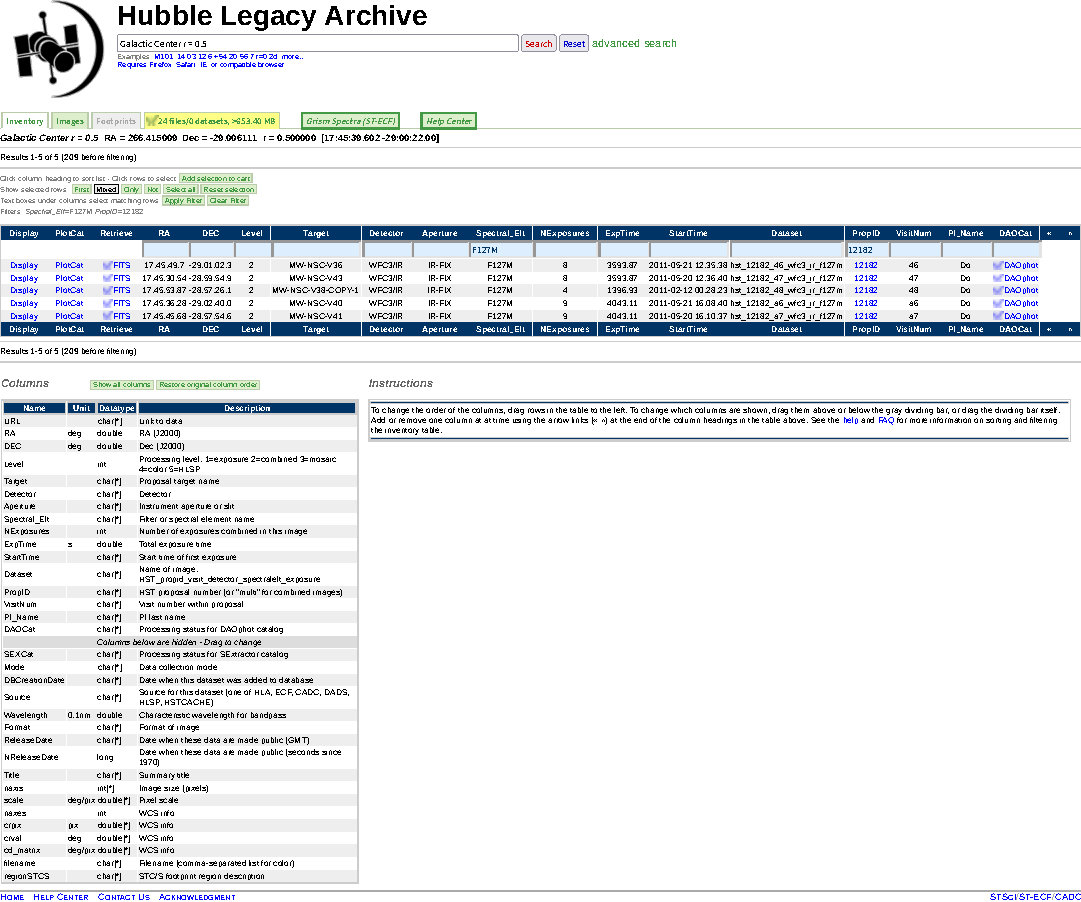
\includegraphics[width=\linewidth,page=1]{img/HLA_screenshot.pdf}
  \caption{Hubble Legacy Archive のスクリーンショット}
  \label{fig:screen:hla}
\end{figure}

\begin{table}
  \centering
  \caption{使用したデータの概要}
  \label{tab:data}
  \small
  \begin{tabular}{cccScc}
    \toprule
    \multicolumn{1}{c}{Filename}
    & \multicolumn{1}{c}{Object}
    & \multicolumn{1}{c}{Filter}
    & \multicolumn{1}{c}{$T_\text{exp}~(\unit{\s})$}
    & \multicolumn{1}{c}{Prop ID}
    & \multicolumn{1}{c}{PI name} \\
    \midrule
    \verb|hst_11671_04_wfc3_ir_f127m_run_1_drz|
    & ARCHES & F127M & 7190.786 & 11671 & Ghez \\
    \verb|hst_11671_04_wfc3_ir_f139m_run_1_drz|
    & ARCHES & F139M & 3492.327 & 11671 & Ghez \\
    \verb|hst_11671_05_wfc3_ir_f127m_run_1_drz|
    & QUINTUPLET & F127M & 7190.786 & 11671 & Ghez \\
    \verb|hst_11671_05_wfc3_ir_f139m_run_1_drz|
    & QUINTUPLET & F139M & 3492.327 & 11671 & Ghez \\
    \verb|hst_11671_06_wfc3_ir_f127m_run_1_drz|
    & SGRA & F127M & 7190.786 & 11671 & Ghez \\
    \verb|hst_11671_06_wfc3_ir_f139m_run_1_drz|
    & SGRA & F139M & 3492.327 & 11671 & Ghez \\
    \verb|hst_12182_46_wfc3_ir_f127m_run_1_drz|
    & MW-NSC-V35 & F127M & 3593.868 & 12182 & Do \\
    \verb|hst_12182_46_wfc3_ir_f139m_run_1_drz|
    & MW-NSC-V35 & F139M & 2193.086 & 12182 & Do \\
    \verb|hst_12182_47_wfc3_ir_f127m_run_1_drz|
    & MW-NSC-V43 & F127M & 3593.868 & 12182 & Do \\
    \verb|hst_12182_47_wfc3_ir_f139m_run_1_drz|
    & MW-NSC-V43 & F139M & 2193.086 & 12182 & Do \\
    \verb|hst_12182_48_wfc3_ir_f127m_run_1_drz|
    & MW-NSC-V38$^\star$ & F127M & 1396.930 & 12182 & Do \\
    \verb|hst_12182_48_wfc3_ir_f139m_run_1_drz|
    & MW-NSC-V38$^\star$ & F139M & 996.927 & 12182 & Do \\
    \verb|hst_12182_a6_wfc3_ir_f127m_run_1_drz|
    & MW-NSC-V37 & F127M & 4043.102 & 12182 & Do \\
    \verb|hst_12182_a6_wfc3_ir_f139m_run_1_drz|
    & MW-NSC-V37 & F139M & 2193.086 & 12182 & Do \\
    \verb|hst_12182_a7_wfc3_ir_f127m_run_1_drz|
     & MW-NSC-V41 & F127M & 4043.102 & 12182 & Do \\
    \verb|hst_12182_a7_wfc3_ir_f139m_run_1_drz|
    & MW-NSC-V41 & F139M & 1993.854 & 12182 & Do \\
    \bottomrule
    \multicolumn{6}{@{}l}{
      \footnotesize$^\star$正確な観測領域名は MW-NSC-V38-COPY-1.}
  \end{tabular}
\end{table}

\subsection{Hubble Space Telescope/Wide Field Camera 3}
WFC3 の装置仕様はウェブ上に詳細なドキュメントが公開されている.\footnote{\url{https://hst-docs.stsci.edu/wfc3ihb}} WFC3 は紫外可視チャンネル (UVIS, two 2k${\times}$4k CCDs, $\ang{;;162}{\times}\ang{;;162}$, $\numrange{200}{1000}\,\si{\nano\meter}$) と赤外線チャンネル (1k${\times}$1k HgCdTe, $\ang{;;136}{\times}\ang{;;123}$, $\numrange{800}{1700}\,\si{\nano\meter}$) をもつ撮像分光観測装置である. HLA から取得したデータはバイアス引き, ダーク引き, フラット補正, バッドピクセル除去, 宇宙線除去, 非線形性補正, Drizzle による合成が完了している. また, FITS ファイルにはサイエンスフレームに加えてキャリブレーションの情報を保存したフレームも含まれている.

サイエンスフレームのカウント値は $\unit{electron\per\second}$ で与えられている. WFC3 の測光システムについてはドキュメントの \href{https://hst-docs.stsci.edu/wfc3dhb/chapter-9-wfc3-data-analysis/9-1-photometry}{9.1 Photometry} で詳細に記述されている. WFC3 の instrumental magnitude は以下の式で定義されている.
\begin{equation}
  m_\text{inst} = -2.5\log{F_\text{count}}.
  \label{eq:wfc3:instmag}
\end{equation}
$F_\text{count}$ はカウントレート ($\unit{electron\per\second}$) である. 物理的な値に変換するために WFC3 Instrument Science Report 2020-10 (\href{https://www.stsci.edu/files/live/sites/www/files/home/hst/instrumentation/wfc3/documentation/instrument-science-reports-isrs/_documents/2020/WFC3-ISR-2020-10.pdf}{Bajaj et al., 2020}) にて報告された等級原点を使用する. 表~\ref{tab:wfc3:zeromag} に今回使用するフィルタの等級原点と変換係数をリストした.

\begin{table}
  \centering
  \caption{HST/WFC3 等級原点リスト (WFC3 ISR 2020-10; Bajaj et al., 2020)}
  \label{tab:wfc3:zeromag}
  \begin{tabular}{ccccccc}
    \toprule
    \multicolumn{1}{c}{Filter}
    & \multicolumn{1}{c}{$\lambda_\text{pivot}$}
    & \multicolumn{1}{c}{$\Delta{\lambda}$}
    & \multicolumn{1}{c}{$M_\text{AB}$}
    & \multicolumn{1}{c}{$M_\text{Vega}$}
    & \multicolumn{1}{c}{$M_\text{ST}$}
    & \multicolumn{1}{c}{$C_{0,\lambda}{}^\star$} \\
    \midrule
    F127M & 12740.29 & 249.56 & 24.6246 & 23.6572 & 26.4584 & \num{9.452e-20} \\
    F139M & 13837.62 & 278.02 & 24.4663 & 23.3815 & 26.4796 & \num{9.313e-20} \\
    \bottomrule
    \multicolumn{7}{@{}l}{\footnotesize$^\star$ $\unit{electron\per\sec}$ から $\unit{erg\per\second\per\square\cm\per\angstrom}$ に変換するための係数.}
  \end{tabular}
\end{table}

\subsection{画像データ}
サンプルとして Arches の画像データを図~\ref{fig:11671:arches} に示した. 左右のパネルに F127M と F139M の画像をそれぞれリニアスケールで表示した. 画像のスケールはどちらも $\numrange{0.5}{2.5}\,\unit{electron\per\second}$ としている. その他の画像は図~\ref{fig:11671}, \ref{fig:12182a} に表示した. いずれの画像もピクセルスケールは $\SI{8.10e-3}{\square\arcsec}$ である. 画像の向きは ICRS 座標系準拠であり, 銀河座標系の座標軸を重ねている.

\begin{figure}
  \centering
  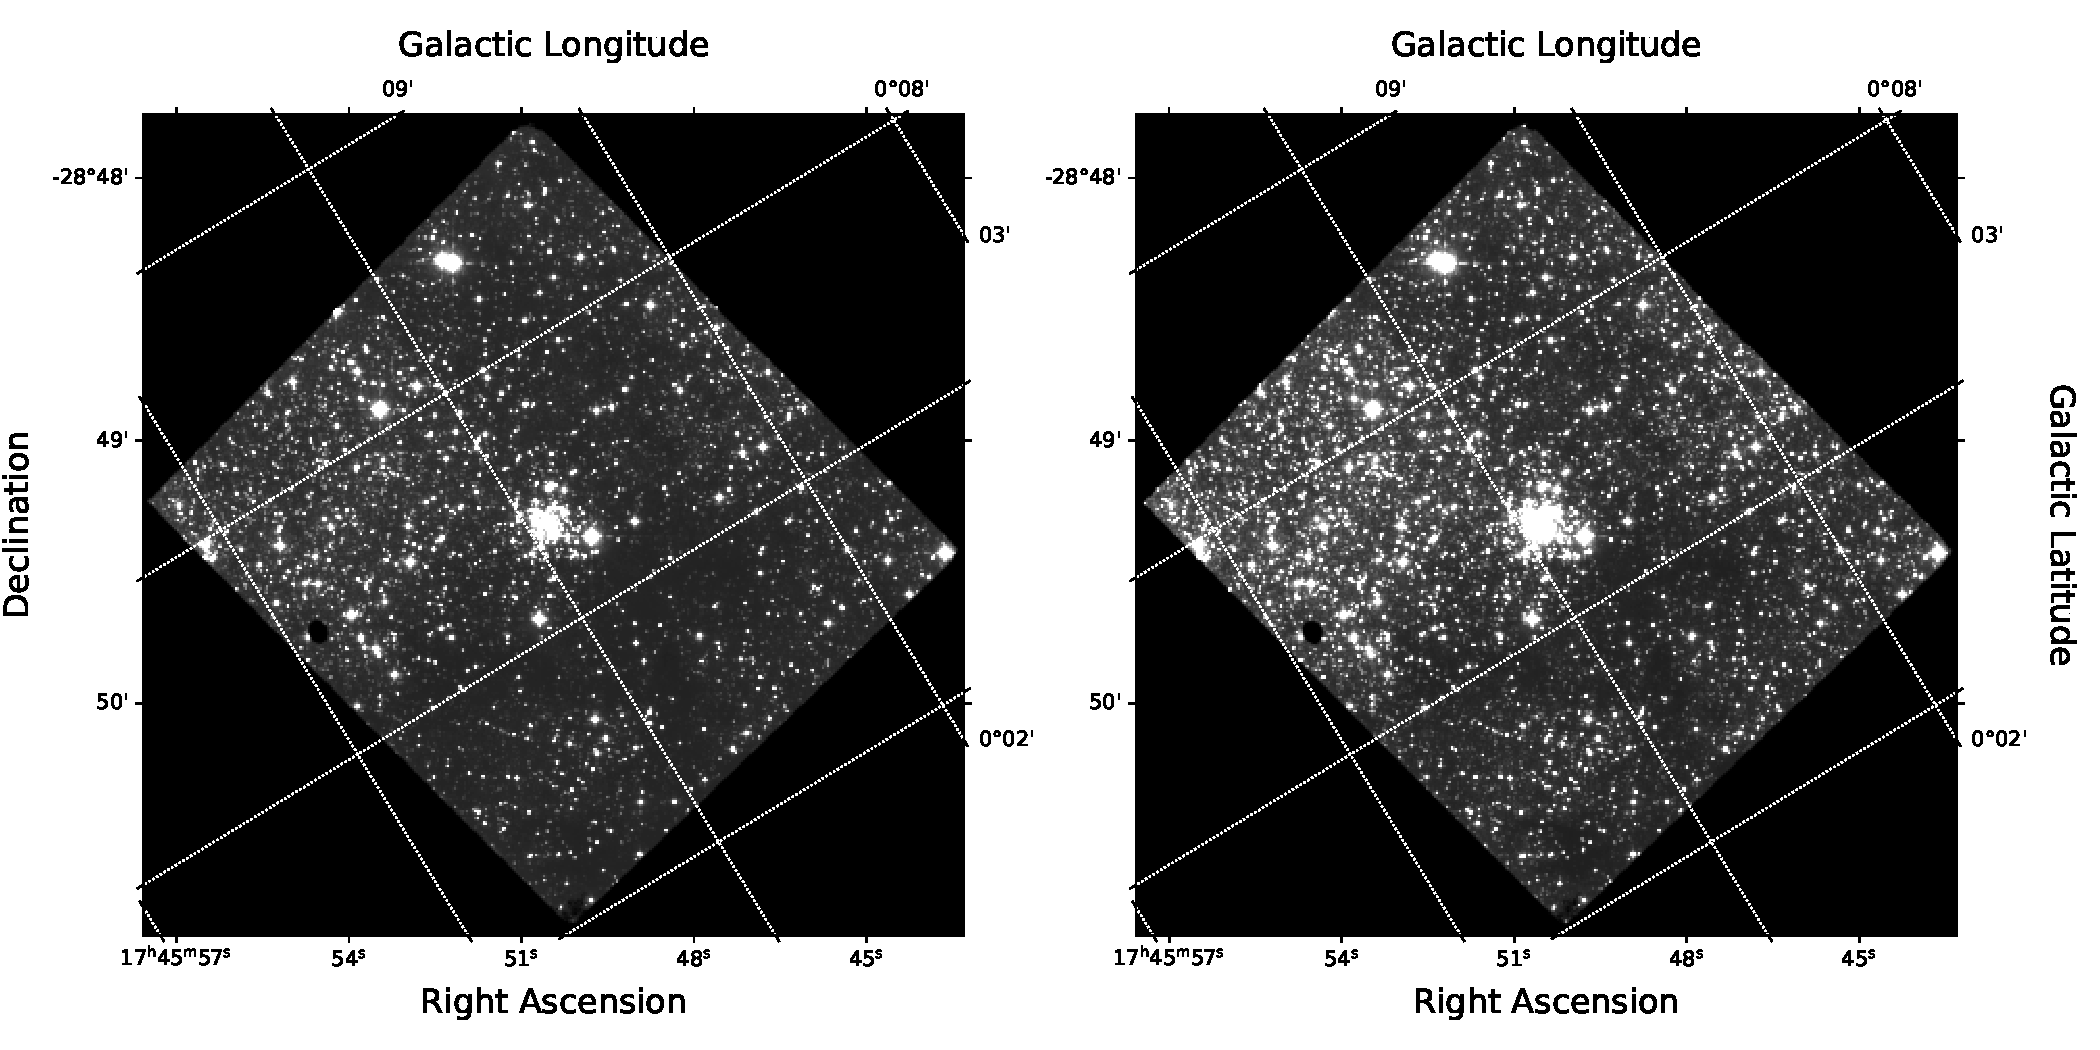
\includegraphics[width=\linewidth]{img/hst_11671_04_wfc3_ir_f127m_drz.pdf}
  \caption{Arches (Prop ID = 11671) の画像データ. 左パネルは F127M の画像, 右パネルは F139M の画像でどちらもリニアスケールで表示している.}
  \label{fig:11671:arches}
\end{figure}

\section{バックグラウンドレベルの評価}
有効画素のヒストグラムからバックグラウンドレベルを評価する. 選定した領域は星の密度が高い領域ではあるが, 総面積としては明るい星以外の領域が大半を占める. そこで画素値のヒストグラムを作成し, ピーク位置から典型的なバックグラウンド放射の強度を推定する.

表~\ref{tab:wfc3:zeromag} に記載された $C_{0,\lambda}$ (\texttt{PHOTFLAM}) とピクセルスケール $\theta$ を使用してカウント値を立体角あたりのエネルギーフラックス密度に変換する.
\begin{equation}
  S_{\lambda} = F_\text{count}\,C_{0,\lambda}/\theta^2.
  \label{eq:conversion}
\end{equation}
図~\ref{fig:histogram:arches} に Arches の画像データから作成したヒストグラムを示す. 上下のパネルはそれぞれ F127M と F139M の画像に対応する. ヒストグラムの幅はどちらも $\SI{1e-18}{J.s^{-1}.m^2.\micro\meter.arcsec^{-2}}$ から $\SI{1e-12}{J.s^{-1}.m^2.\micro\meter.arcsec^{-2}}$ までを等間隔に 400 等分している. ヒストグラムのピーク値を典型的なバックグラウンド放射の強度として見積もった. 計算したピーク位置をオレンジ色の破線で示している. 同じ操作をすべての領域におこない, バックグラウンド放射の強度をそれぞれ導出した. 計算した結果を表~\ref{tab:brightness} にまとめた. 他の領域のヒストグラムは図~\ref{fig:histogram:1} にまとめて表示している.

\begin{figure}
  \centering
  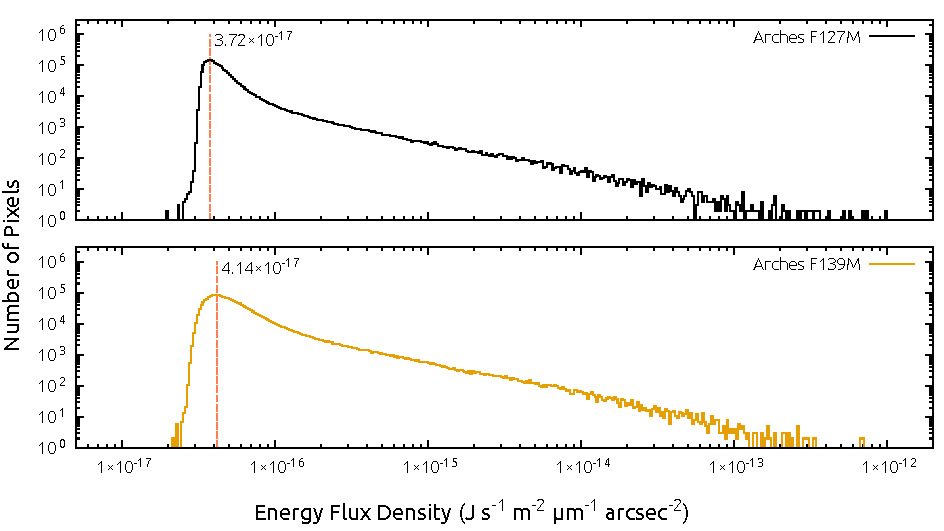
\includegraphics[width=\linewidth,page=1]{img/histogram.pdf}
  \caption{Arches の画像データを元に作成した面輝度のヒストグラム. 上下のパネルはそれぞれ F127M と F139M の画像を使用して作成した. 推定したピーク位置を破線で示した.}
  \label{fig:histogram:arches}
\end{figure}

\begin{table}
  \centering
  \caption{推定したバックグラウンド放射強度}
  \label{tab:brightness}
  \small
  \begin{tabular}{c
    S[table-format=1.2e2]
    S[table-format=1.2e2]
    S[table-format=3.2]
    S[table-format=3.2]
    S[table-format=2.2]
    S[table-format=2.2]}
    \toprule
    \multicolumn{1}{c}{}
    & \multicolumn{2}{c}{Energy Flux Density$^\star$}
    & \multicolumn{2}{c}{Photon Flux Density$^\dagger$}
    & \multicolumn{2}{c}{Electron Count Rate$^\ddagger$} \\
    \multicolumn{1}{c}{Object}
    & \multicolumn{1}{c}{F127M}
    & \multicolumn{1}{c}{F139M}
    & \multicolumn{1}{c}{\footnotesize\numrange{1.1}{1.6}\,\unit{\micro\meter}}
    & \multicolumn{1}{c}{\footnotesize\numrange{0.9}{1.6}\,\unit{\micro\meter}}
    & \multicolumn{1}{c}{\footnotesize\numrange{1.1}{1.6}\,\unit{\micro\meter}}
    & \multicolumn{1}{c}{\footnotesize\numrange{0.9}{1.6}\,\unit{\micro\meter}} \\
    \midrule
    Arches     & 3.72e-17 & 4.14e-17 & 139.35 & 168.25 & 2.05 & 2.48 \\
    Quintuplet & 4.53e-17 & 5.90e-17 & 203.12 & 227.15 & 2.99 & 3.35 \\
    SGRA       & 5.46e-17 & 1.03e-16 & 431.19 & 443.28 & 6.36 & 6.54 \\
    MW-NSC-V35 & 4.09e-17 & 4.73e-17 & 159.49 & 188.48 & 2.35 & 2.78 \\
    MW-NSC-V43 & 5.28e-17 & 7.79e-17 & 280.64 & 301.44 & 4.14 & 4.44 \\
    MW-NSC-V38 & 6.78e-17 & 8.21e-17 & 278.53 & 321.29 & 4.11 & 4.74 \\
    MW-NSC-V37 & 3.91e-17 & 5.39e-17 & 188.88 & 206.91 & 2.78 & 3.05 \\
    MW-NSC-V41 & 4.88e-17 & 6.85e-17 & 241.70 & 263.33 & 3.56 & 3.88 \\
    \bottomrule
    \multicolumn{7}{@{}l}{
      \footnotesize$^\star$
      in units of \si{J.s^{-1}.m^{-2}.\micro m^{-1}.arcsec^{-2}}} \\
    \multicolumn{7}{@{}l}{
      \footnotesize$^\dagger$
      integrated over JASMINE's photometric band;
      in units of \si{photon.s^{-1}.m^{-2}.arcsec^{-2}}} \\
      \multicolumn{7}{@{}l}{
        \footnotesize$^\ddagger$
        integrated over JASMINE's photometric band;
        in units of \si{electron.s^{-1}.pixel^{-1}}}
      \end{tabular}
\end{table}

推定したエネルギーフラックス密度を JASMINE の観測波長帯でのフォトンフラックスに換算する. 簡単のためにバックグラウンド放射が等級空間 (対数空間) で波長に対して線形であると仮定する. 表~\ref{tab:brightness} に記載した $\SI{1.274}{\micro\meter}$ と $\SI{1.384}{\micro\meter}$ の推定値からバックグラウンド放射の SED を以下のように定義する.
\begin{equation}
  S_{\lambda,\text{BG}}(\lambda) =
  \exp(
    \frac{\lambda_\text{F135M}-\lambda}{\lambda_\text{F135M}-\lambda_\text{F127M}}
    \log{S_{\lambda,\text{F127M}}}
    +\frac{\lambda-\lambda_\text{F129M}}{\lambda_\text{F135M}-\lambda_\text{F127M}}
    \log{S_{\lambda,\text{F139M}}}
  ).
  \label{eq:sed}
\end{equation}
$\lambda_\text{X}$, $S_{\lambda,\text{X}}$ はそれぞれは観測フィルタ X の有効波長とバックグラウンド放射強度である. 光子数に変換して JASMINE の観測波長帯域で積分することで, 実効的なフォトンフラックス面密度を計算する.
\begin{equation}
  S^\text{photon}_\text{BG}
  = \int S_{\lambda,\text{BG}}(\lambda) \frac{\lambda}{hc} \dd{\lambda}
\end{equation}
JASMINE の観測波長として \numrange{1.1}{1.6}\,\unit{\micro\meter} を仮定したケースと \numrange{0.9}{1.6}\,\unit{\micro\meter} を仮定したケースをそれぞれ表~\ref{tab:brightness} に記載した. 単位は \unit{photon.s^{-1}.m^{-2}.arcsec^{-2}} である.

JASMINE の観測においてピクセルあたり検出する電子数を見積もる. ピクセルスケールを \SI{0.424}{arcsec}, 主鏡の有効直径を \SI{40}{\centi\meter} とする. 光学系の効率を $0.97^5 = 0.86$, フィルタの透過率を 0.95, 検出器の量子効率を 0.8 とする. バックグラウンド放射から期待される電子の発生レートを表~\ref{tab:brightness} にまとめた. 現在想定している InGaAs 検出器のダークカレントは \SI{15.5}{electron.s^{-1}.pixel^{-1}} である. 今回調査した中で最も電子の発生レートが高かったのは SGRA 領域の \SI{6.54}{electron.s^{-1}.pixel} である. これは検出器のダークカレントに対して \SI{40}{\percent} 程度のレートであり, バックグラウンド放射の寄与はダークカレントを上回ることはなさそうであるが, 無視できない程度の寄与になると考えられる.


\appendix
\section{画像データ}
\subsection{HST/WFC3 画像データ}
この資料で使用した画像データを図~\ref{fig:11671}, \ref{fig:12182a} に表示する. 画像の説明はいずれも図~\ref{fig:11671:arches} と同様である.

\begin{figure}
  \centering
  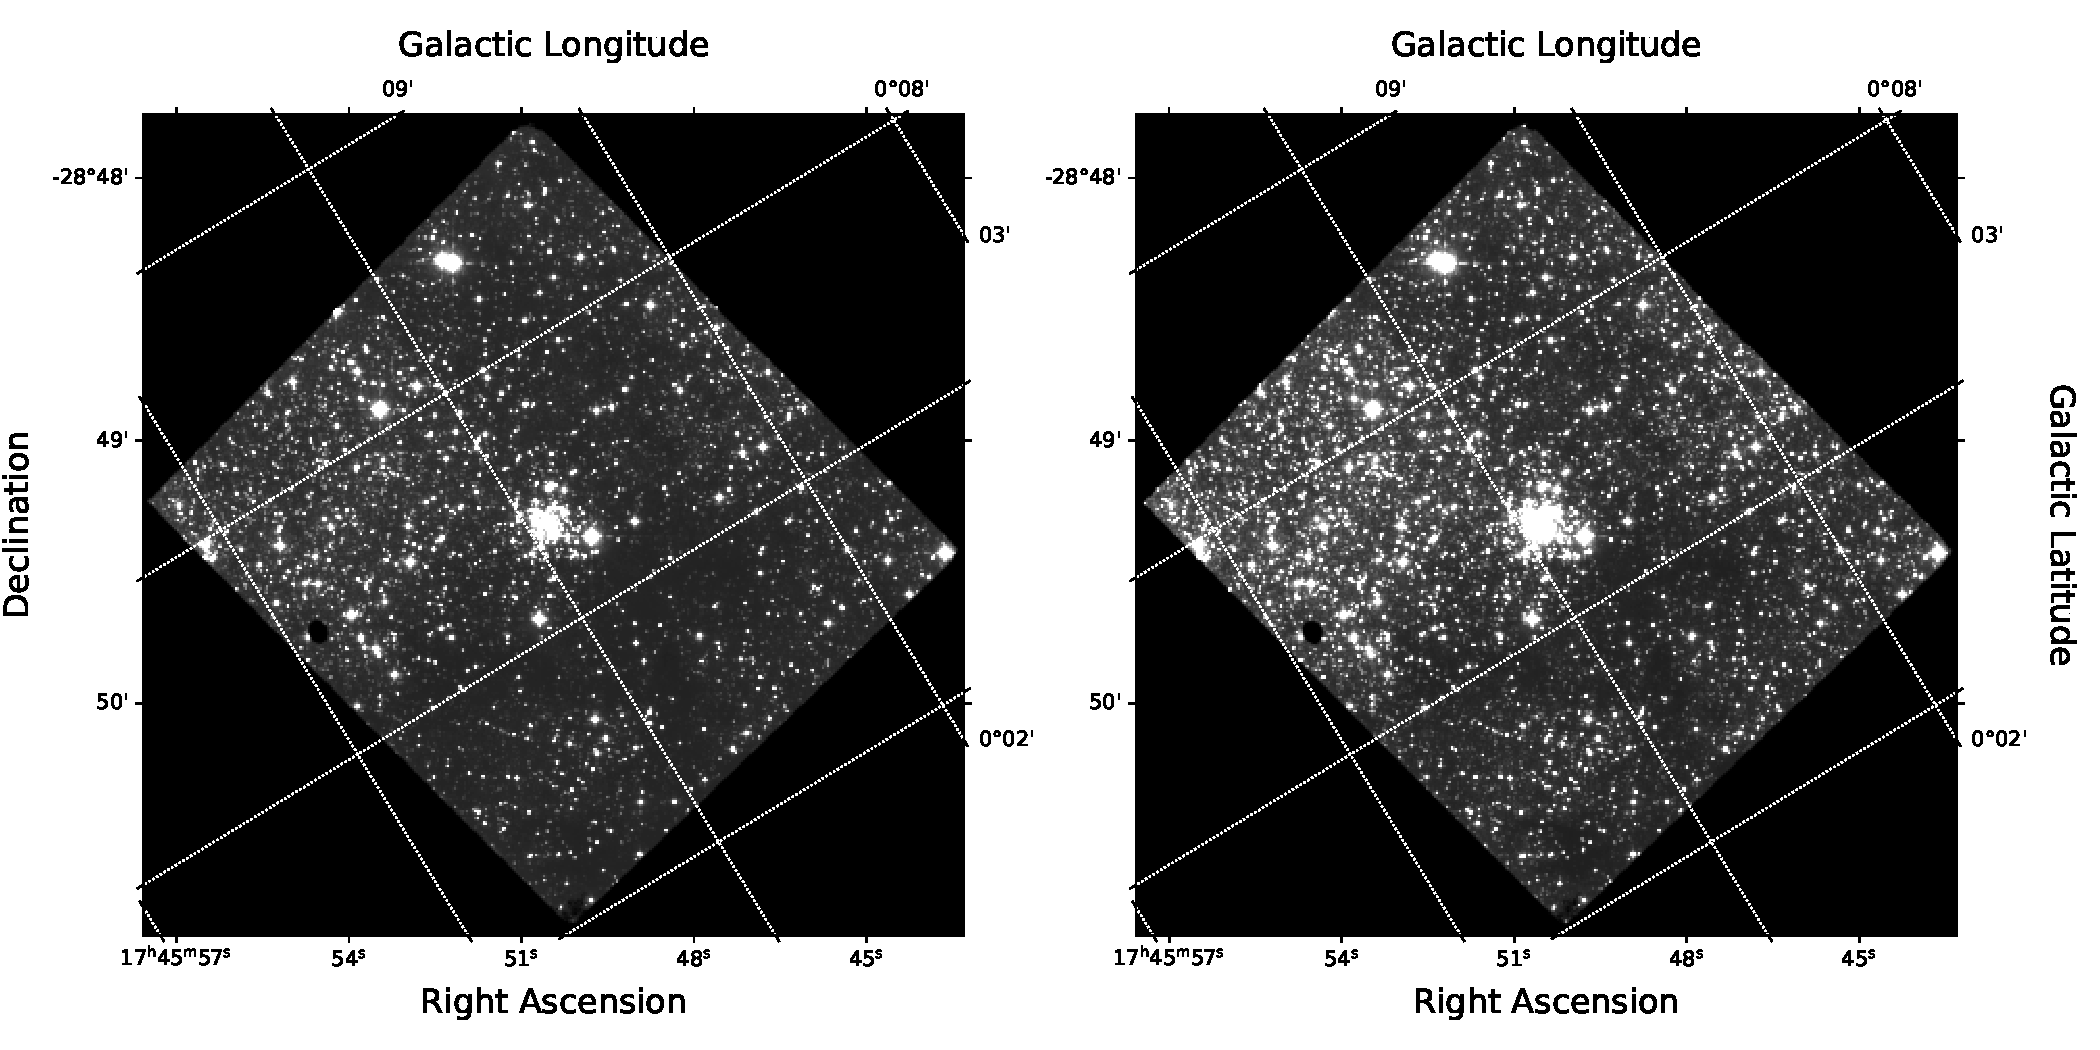
\includegraphics[width=\linewidth]{img/hst_11671_04_wfc3_ir_f127m_drz.pdf}
  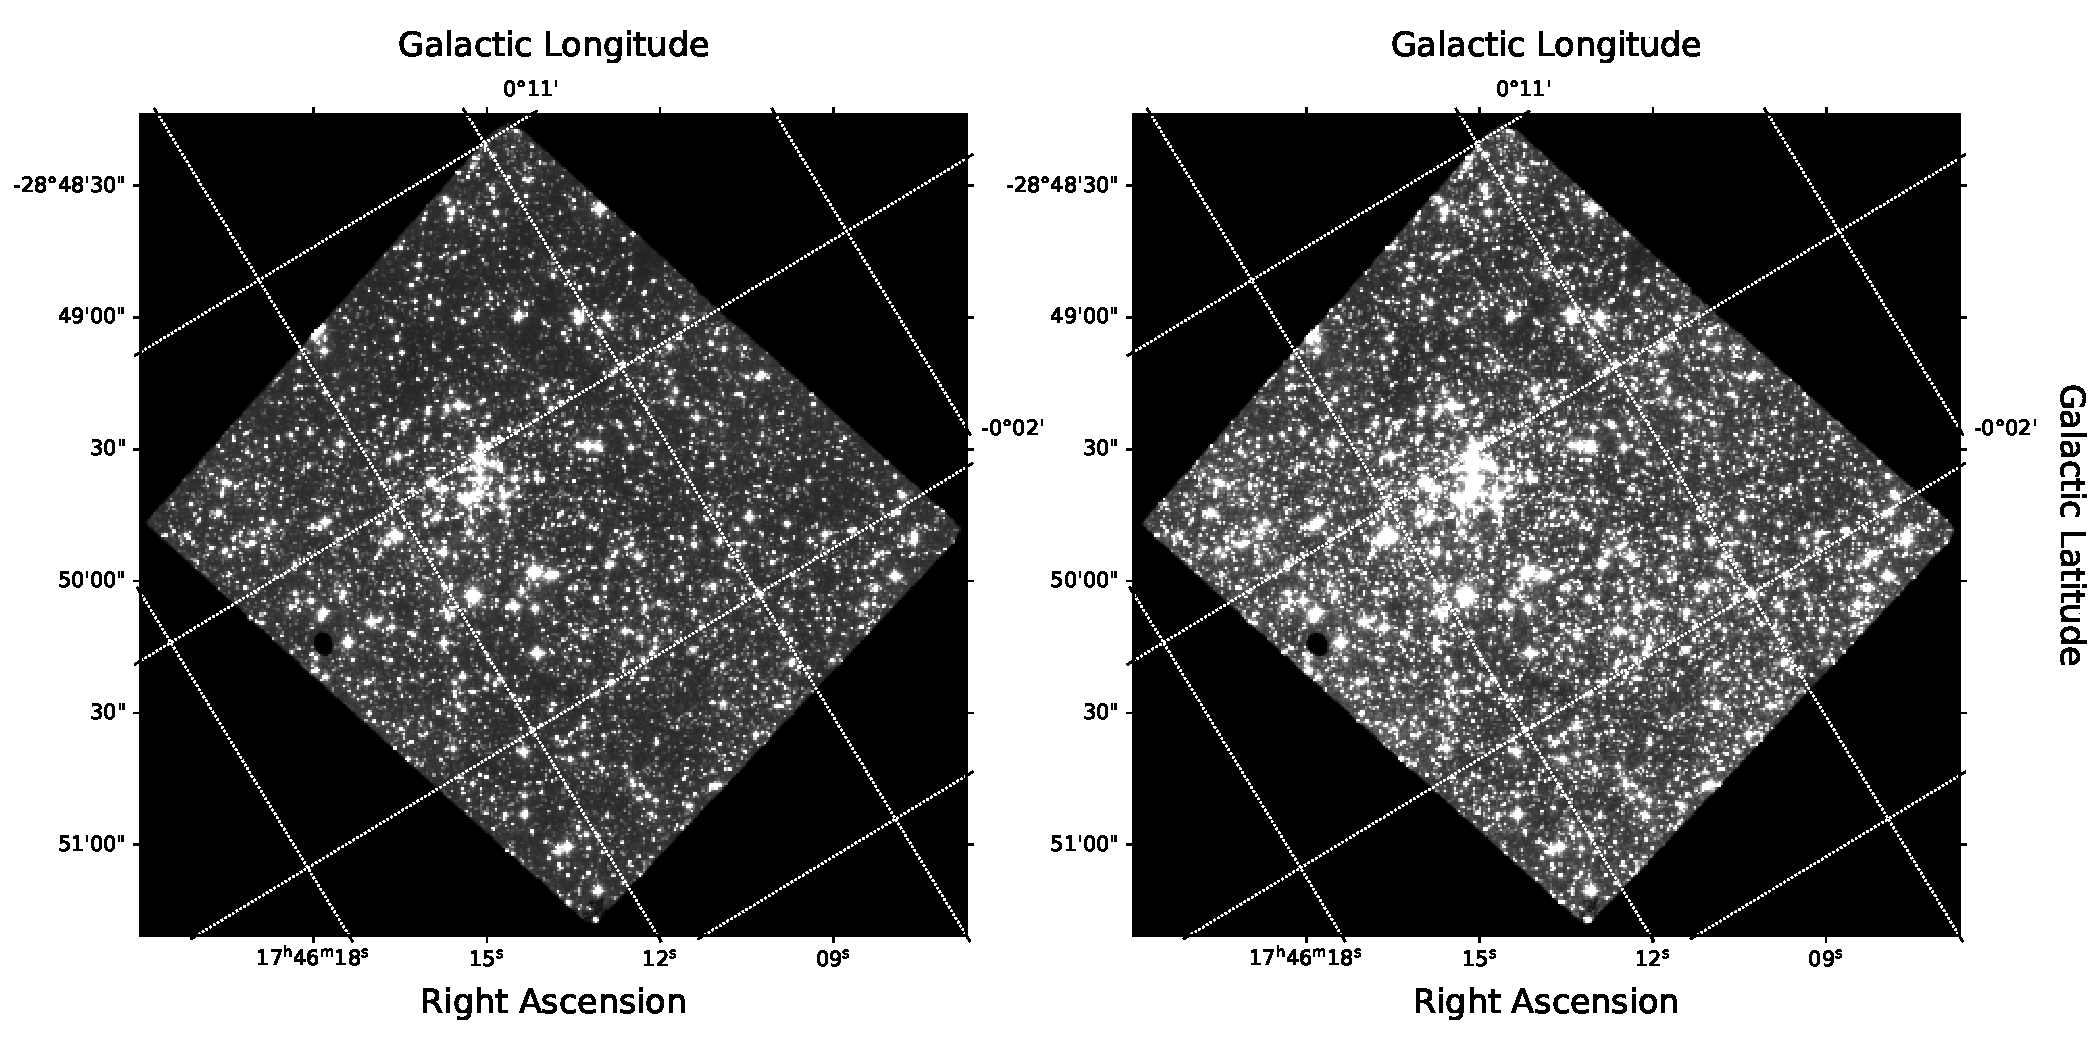
\includegraphics[width=\linewidth]{img/hst_11671_05_wfc3_ir_f127m_drz.pdf}
  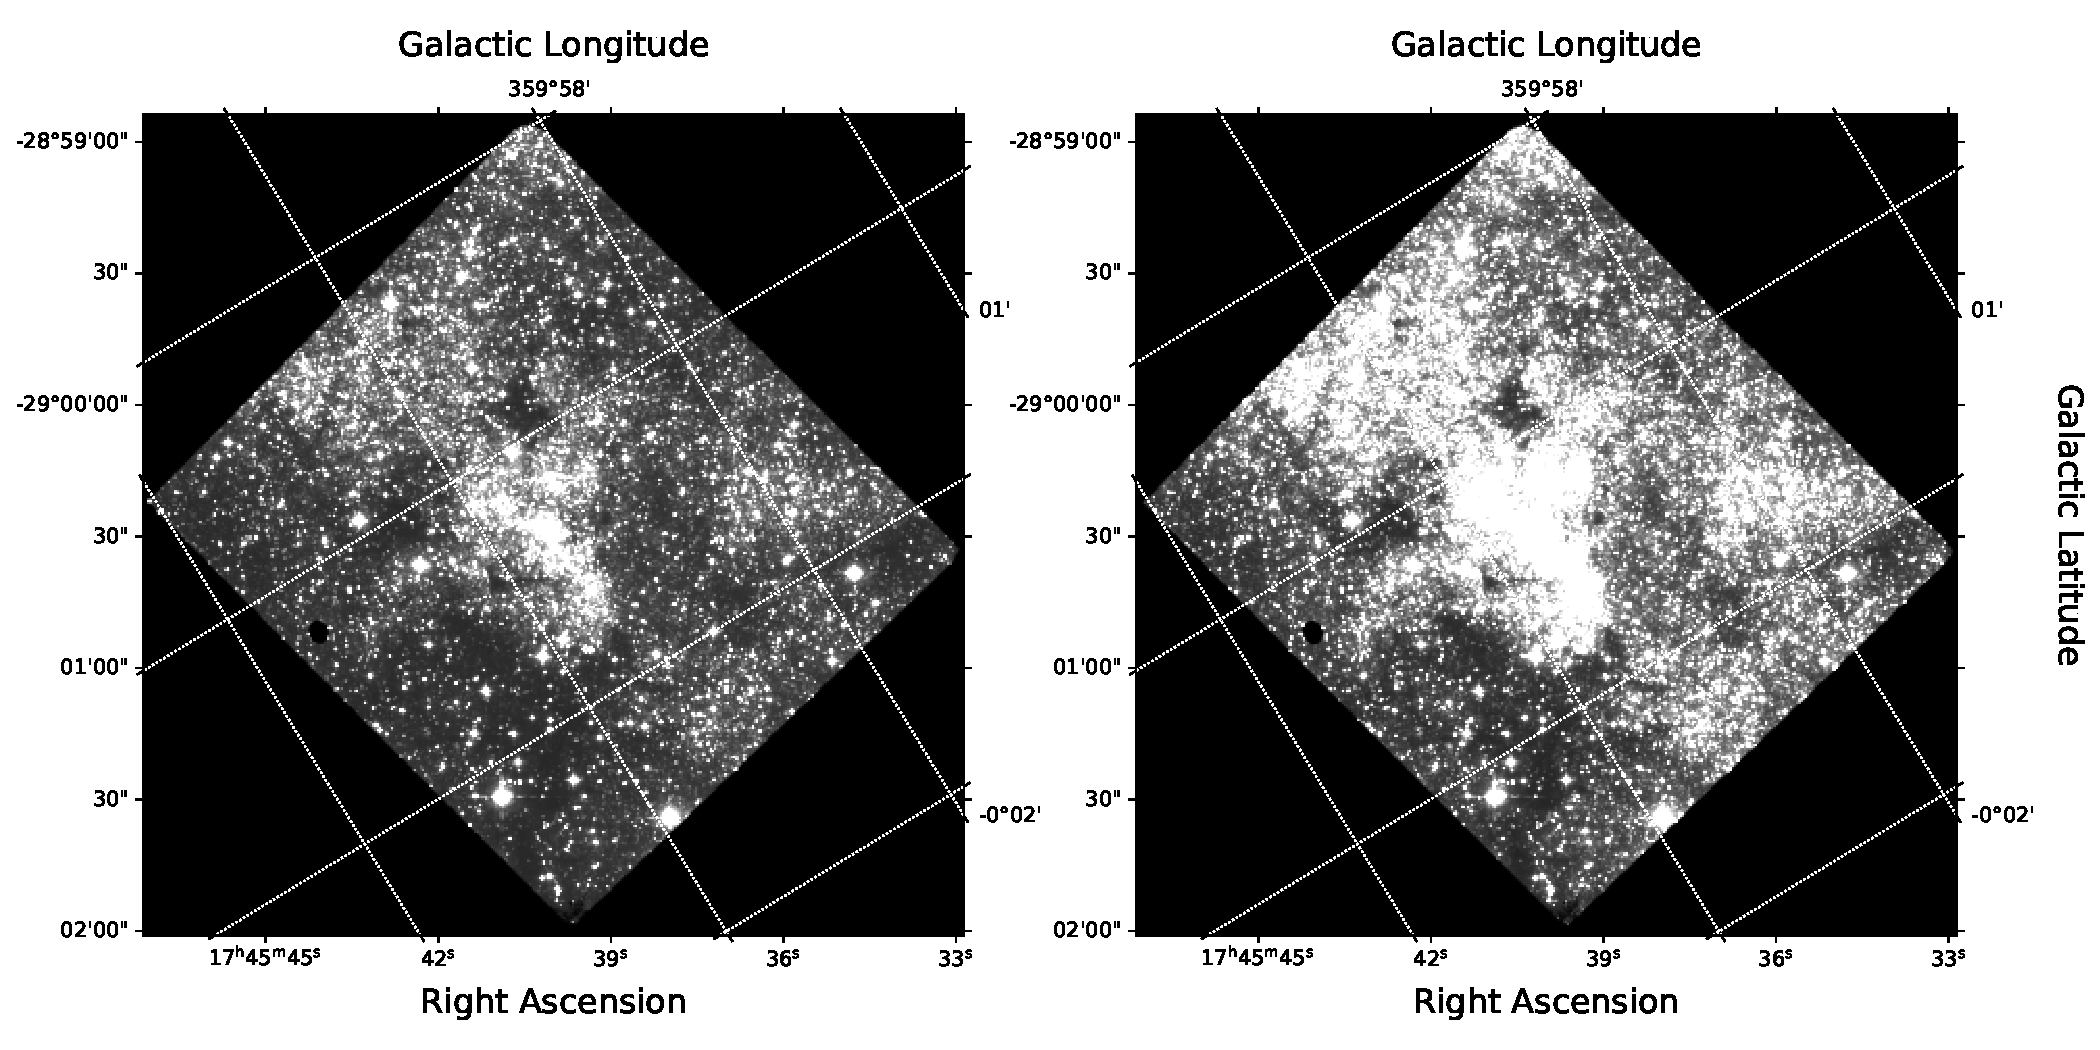
\includegraphics[width=\linewidth]{img/hst_11671_06_wfc3_ir_f127m_drz.pdf}
  \caption{Proposal ID 11671 の画像データ. 左パネルは F127M の画像, 右パネルは F139M の画像でどちらもリニアスケールで表示している. 上から順番に Arches, Quintuplet, SGRA の領域を示す.}
  \label{fig:11671}
\end{figure}

\begin{figure}
  \centering
  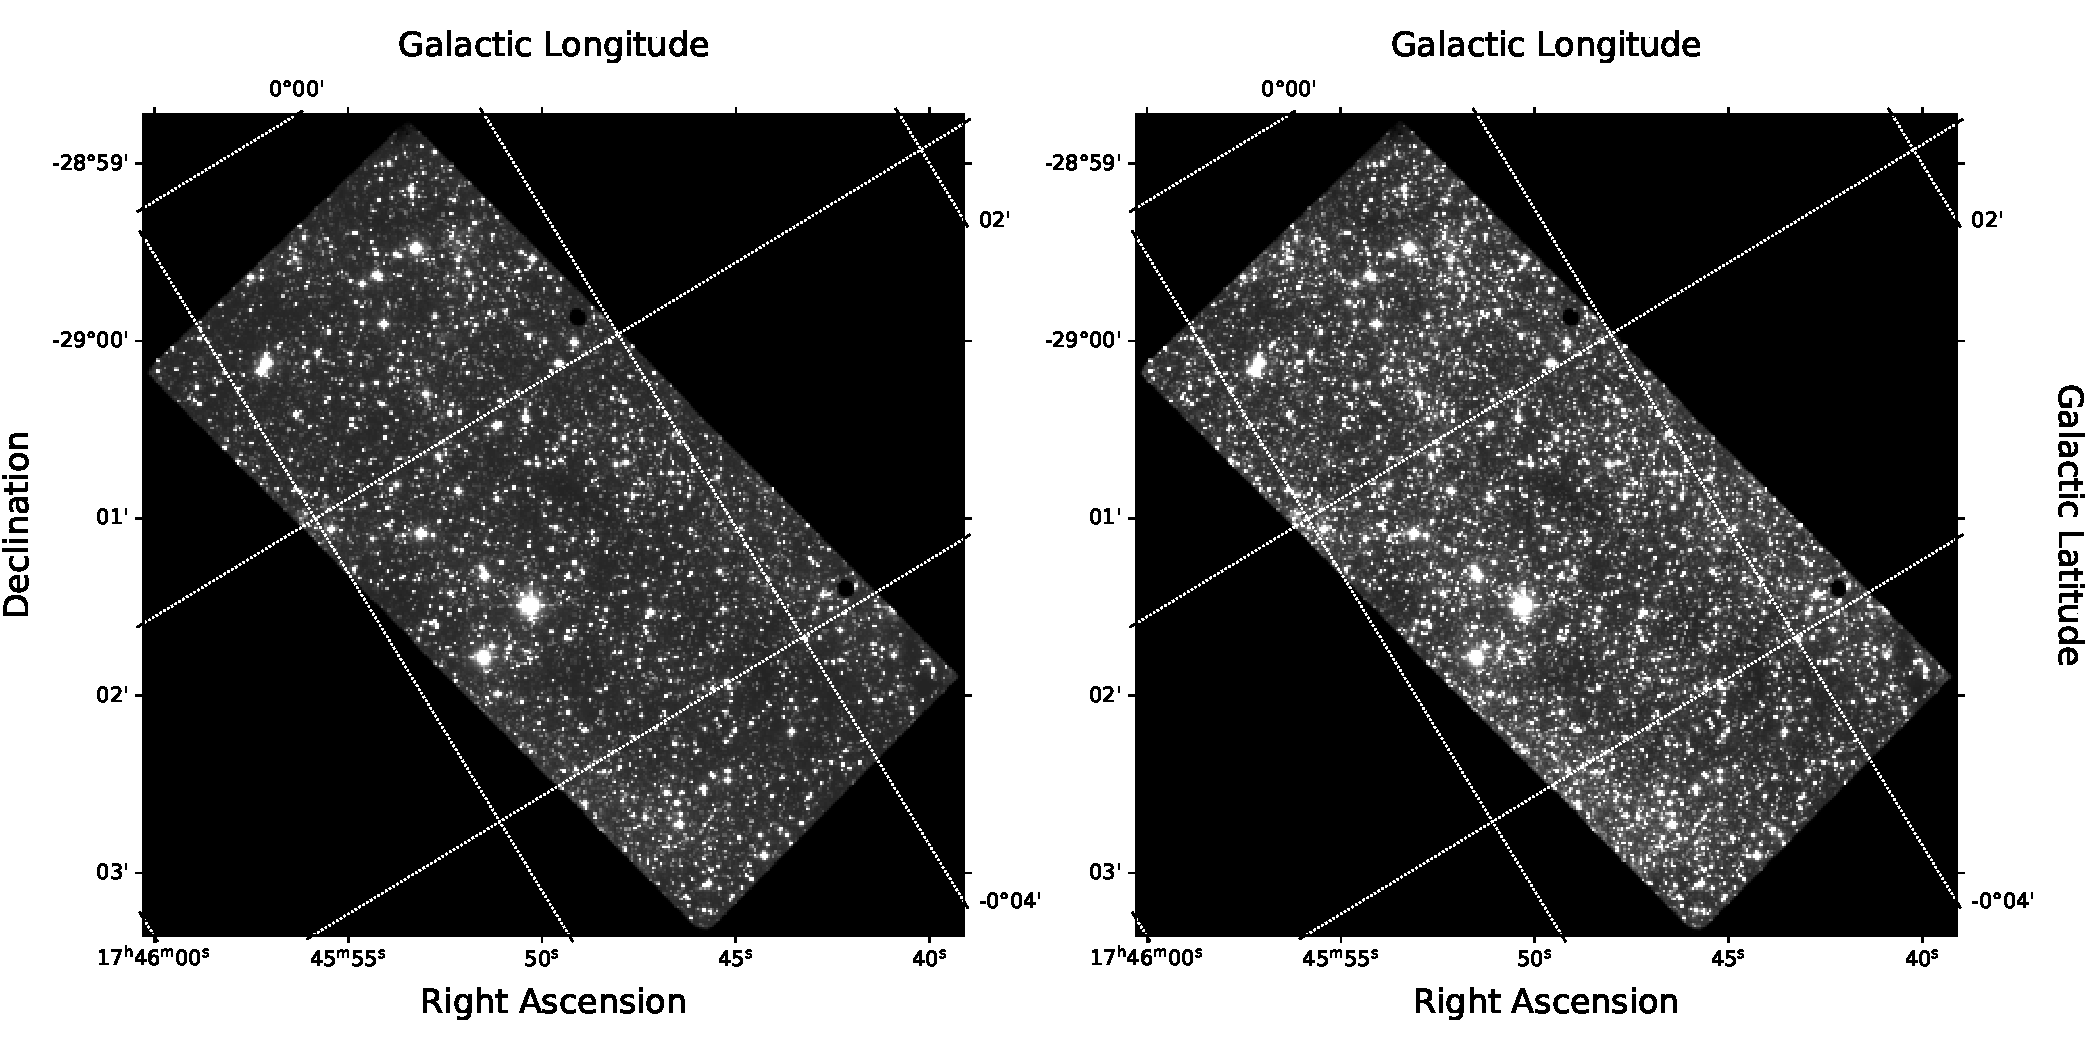
\includegraphics[width=\linewidth]{img/hst_12182_46_wfc3_ir_f127m_drz.pdf}
  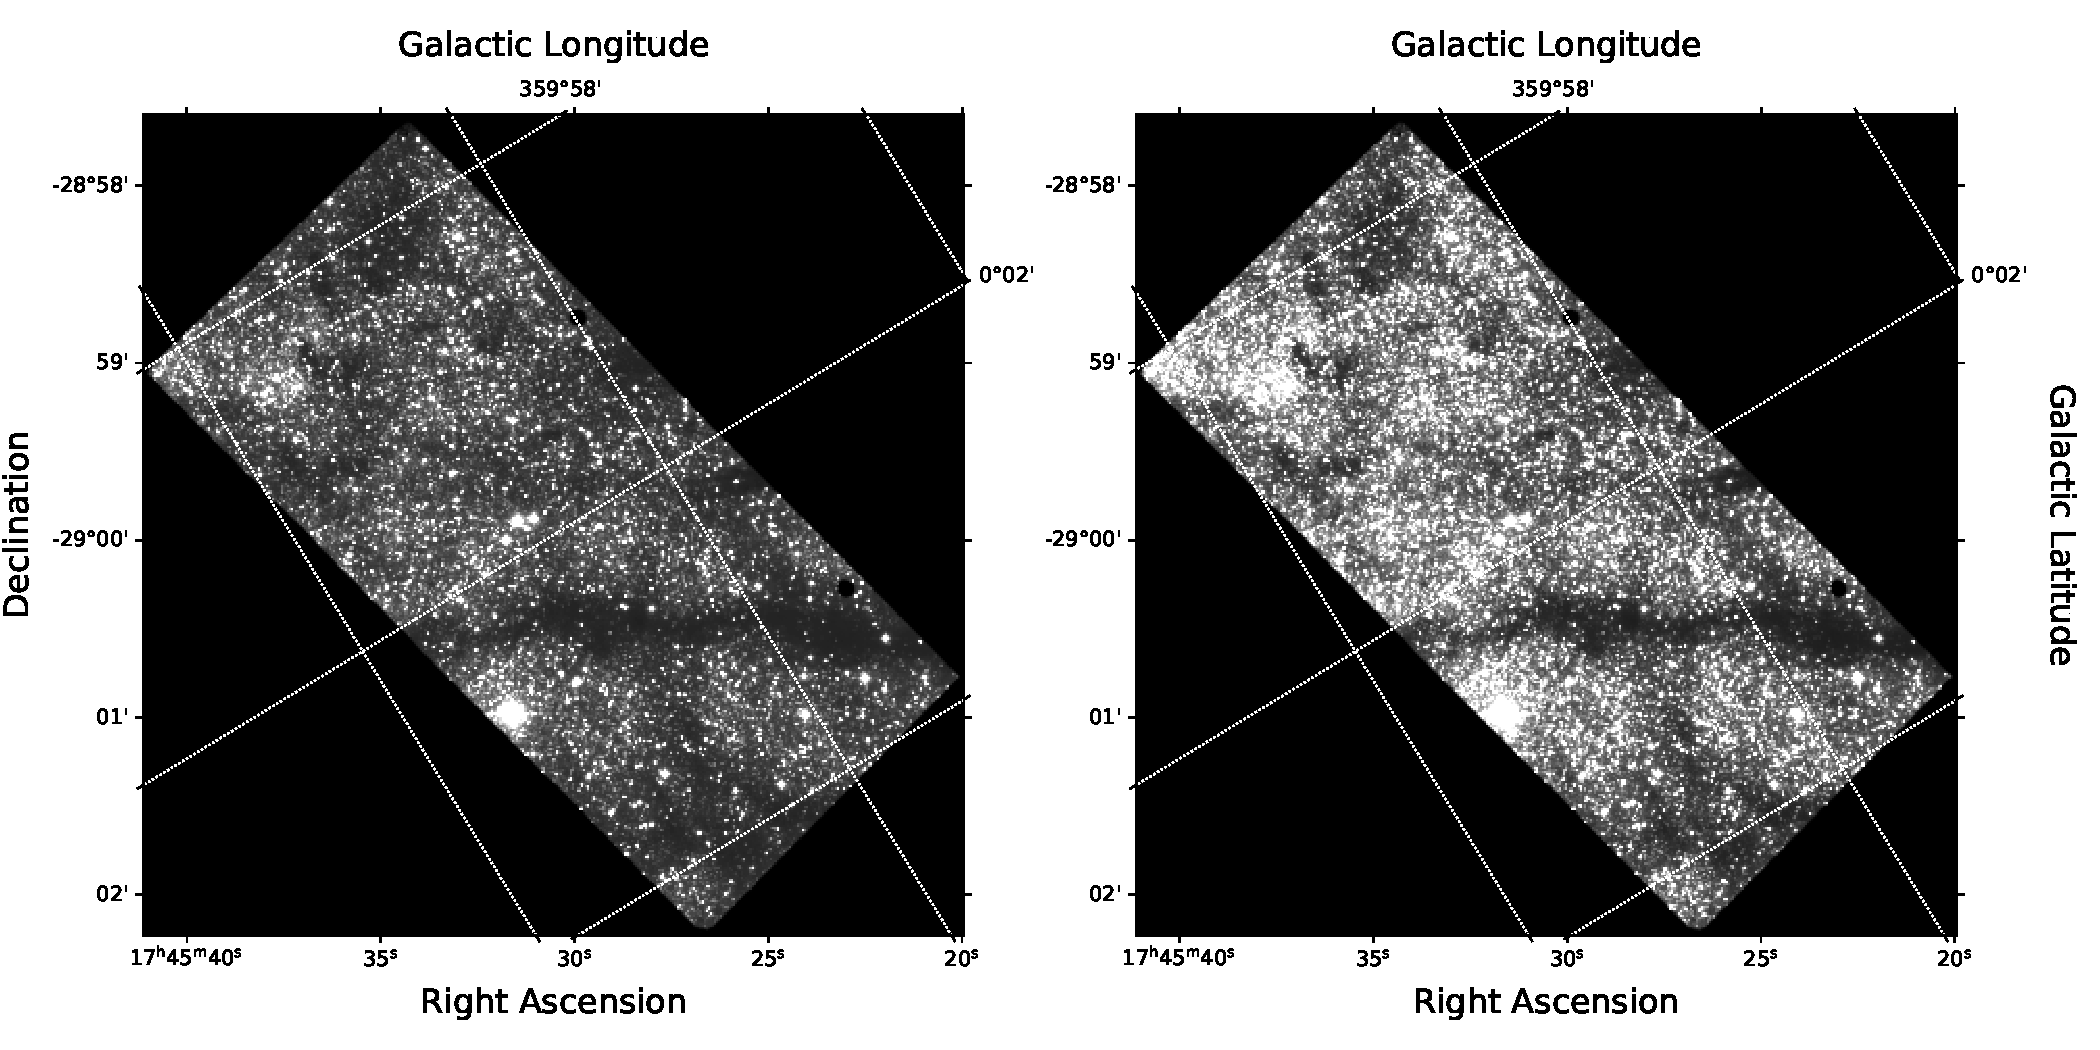
\includegraphics[width=\linewidth]{img/hst_12182_47_wfc3_ir_f127m_drz.pdf}
  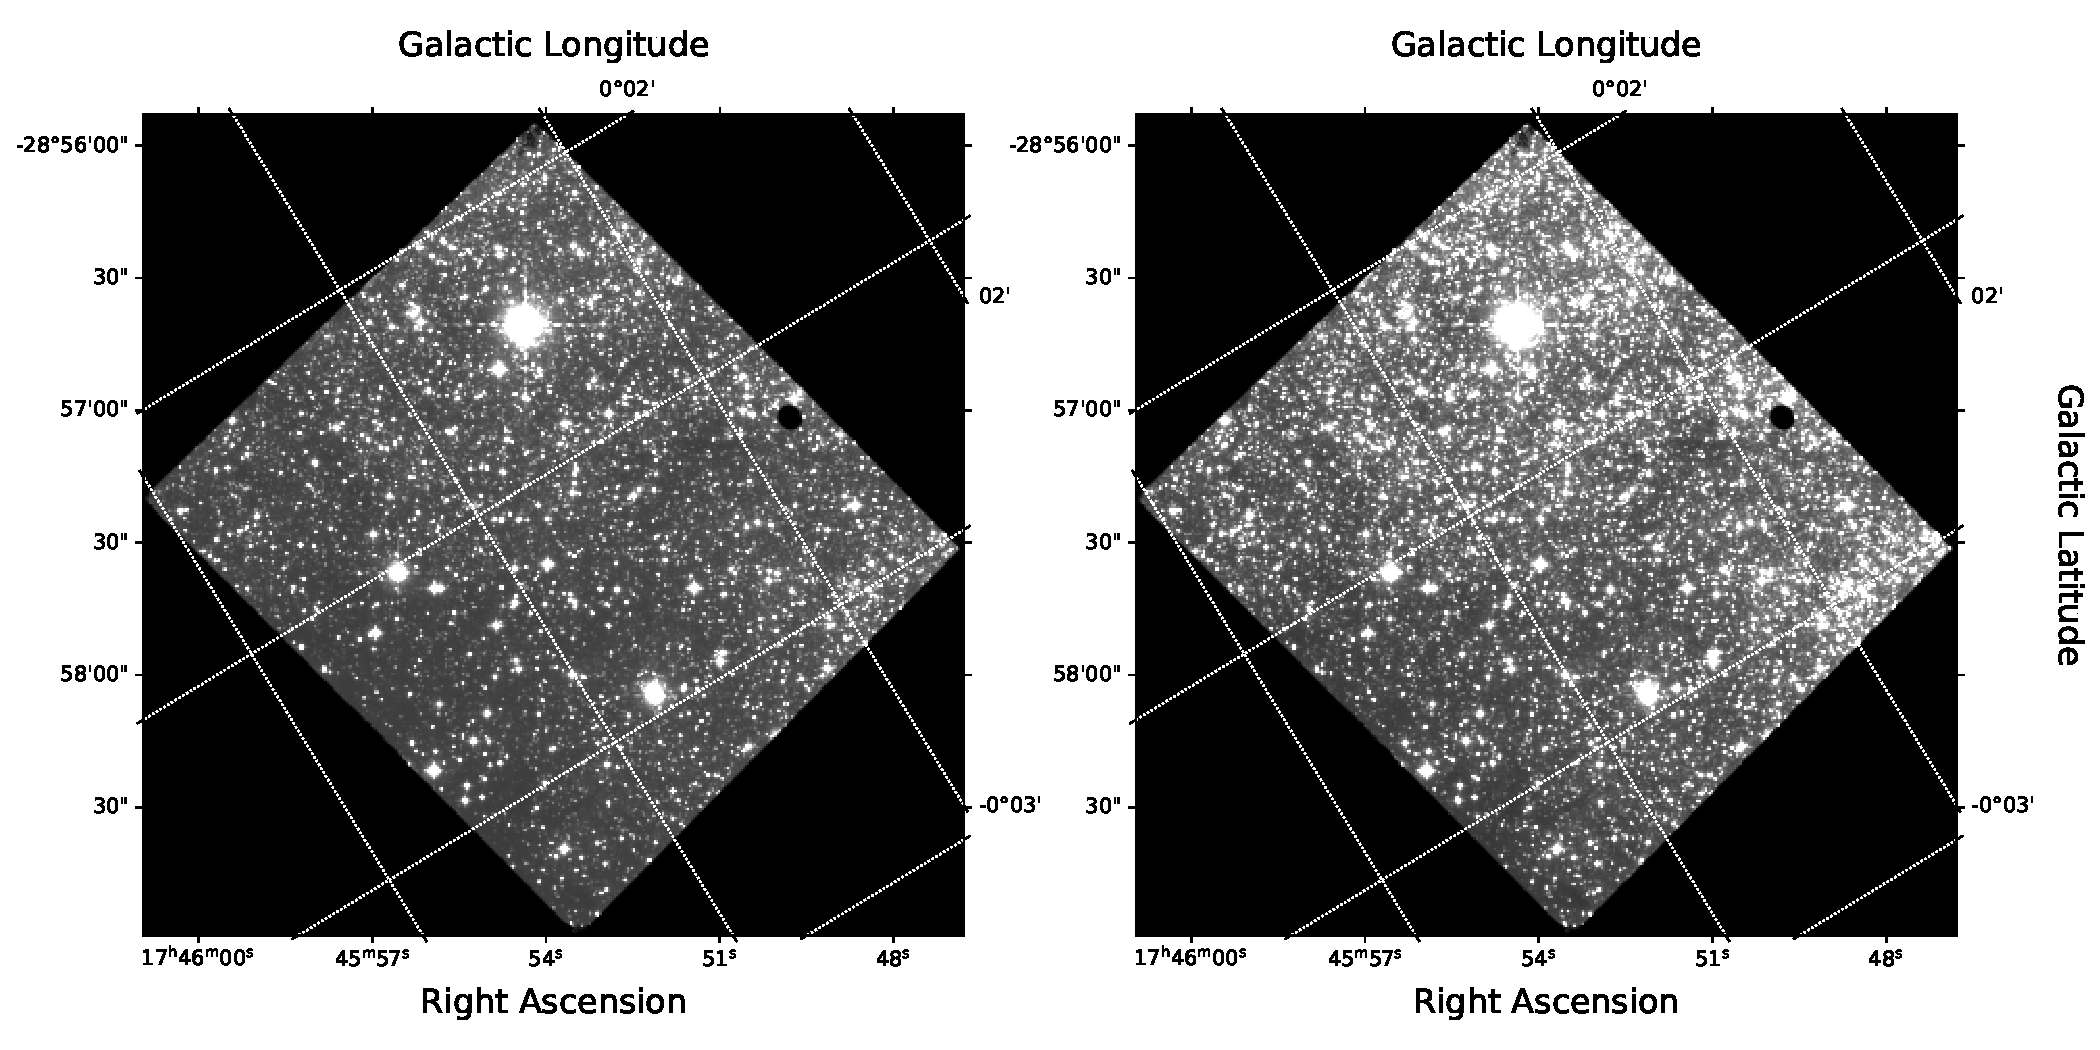
\includegraphics[width=\linewidth]{img/hst_12182_48_wfc3_ir_f127m_drz.pdf}
  \caption{Proposal ID 12182 の画像データ. 左パネルは F127M の画像, 右パネルは F139M の画像でどちらもリニアスケールで表示している. 上から順番に MW-NSC-V35, MW-NSC-V43, MW-NSC-V38 の領域を示す.}
  \label{fig:12182a}
\end{figure}

\addtocounter{figure}{-1}
\begin{figure}
  \centering
  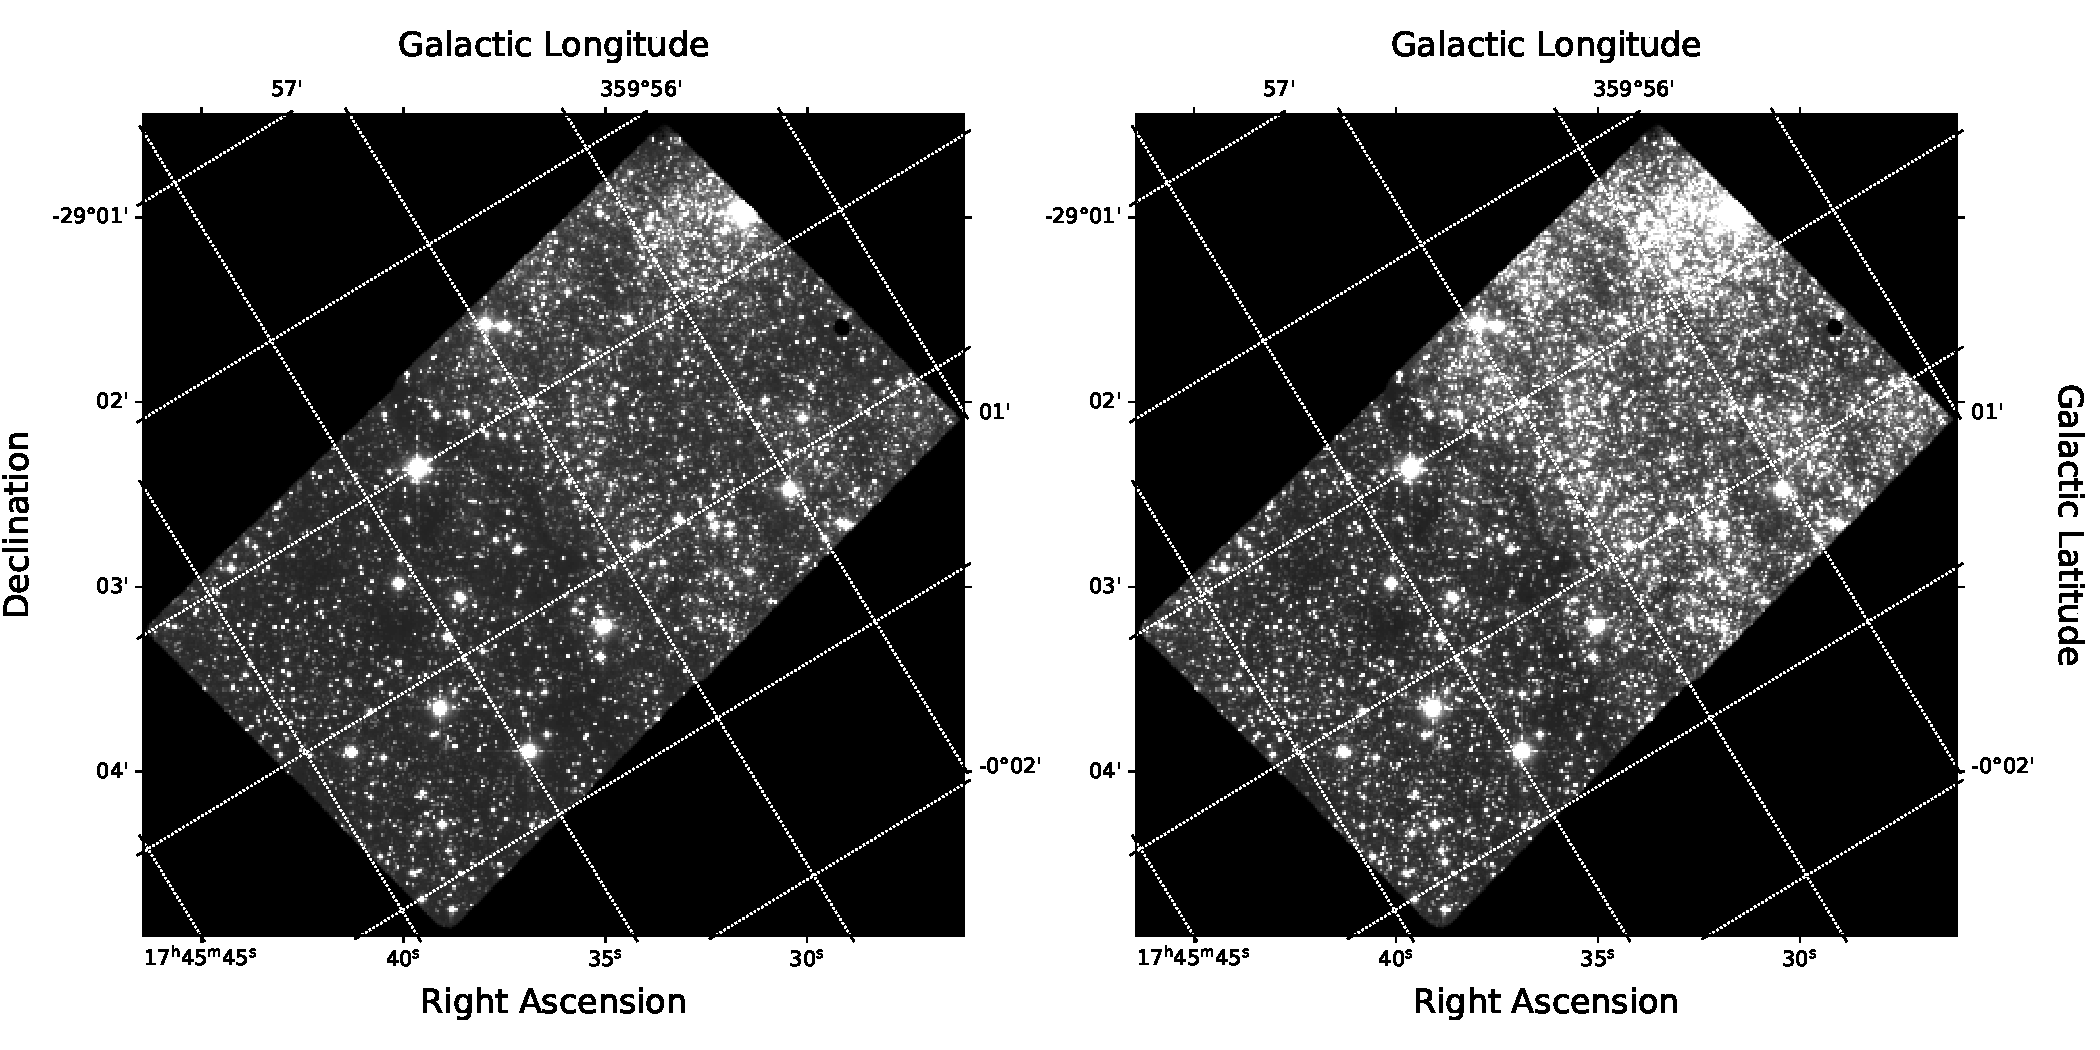
\includegraphics[width=\linewidth]{img/hst_12182_a6_wfc3_ir_f127m_drz.pdf}
  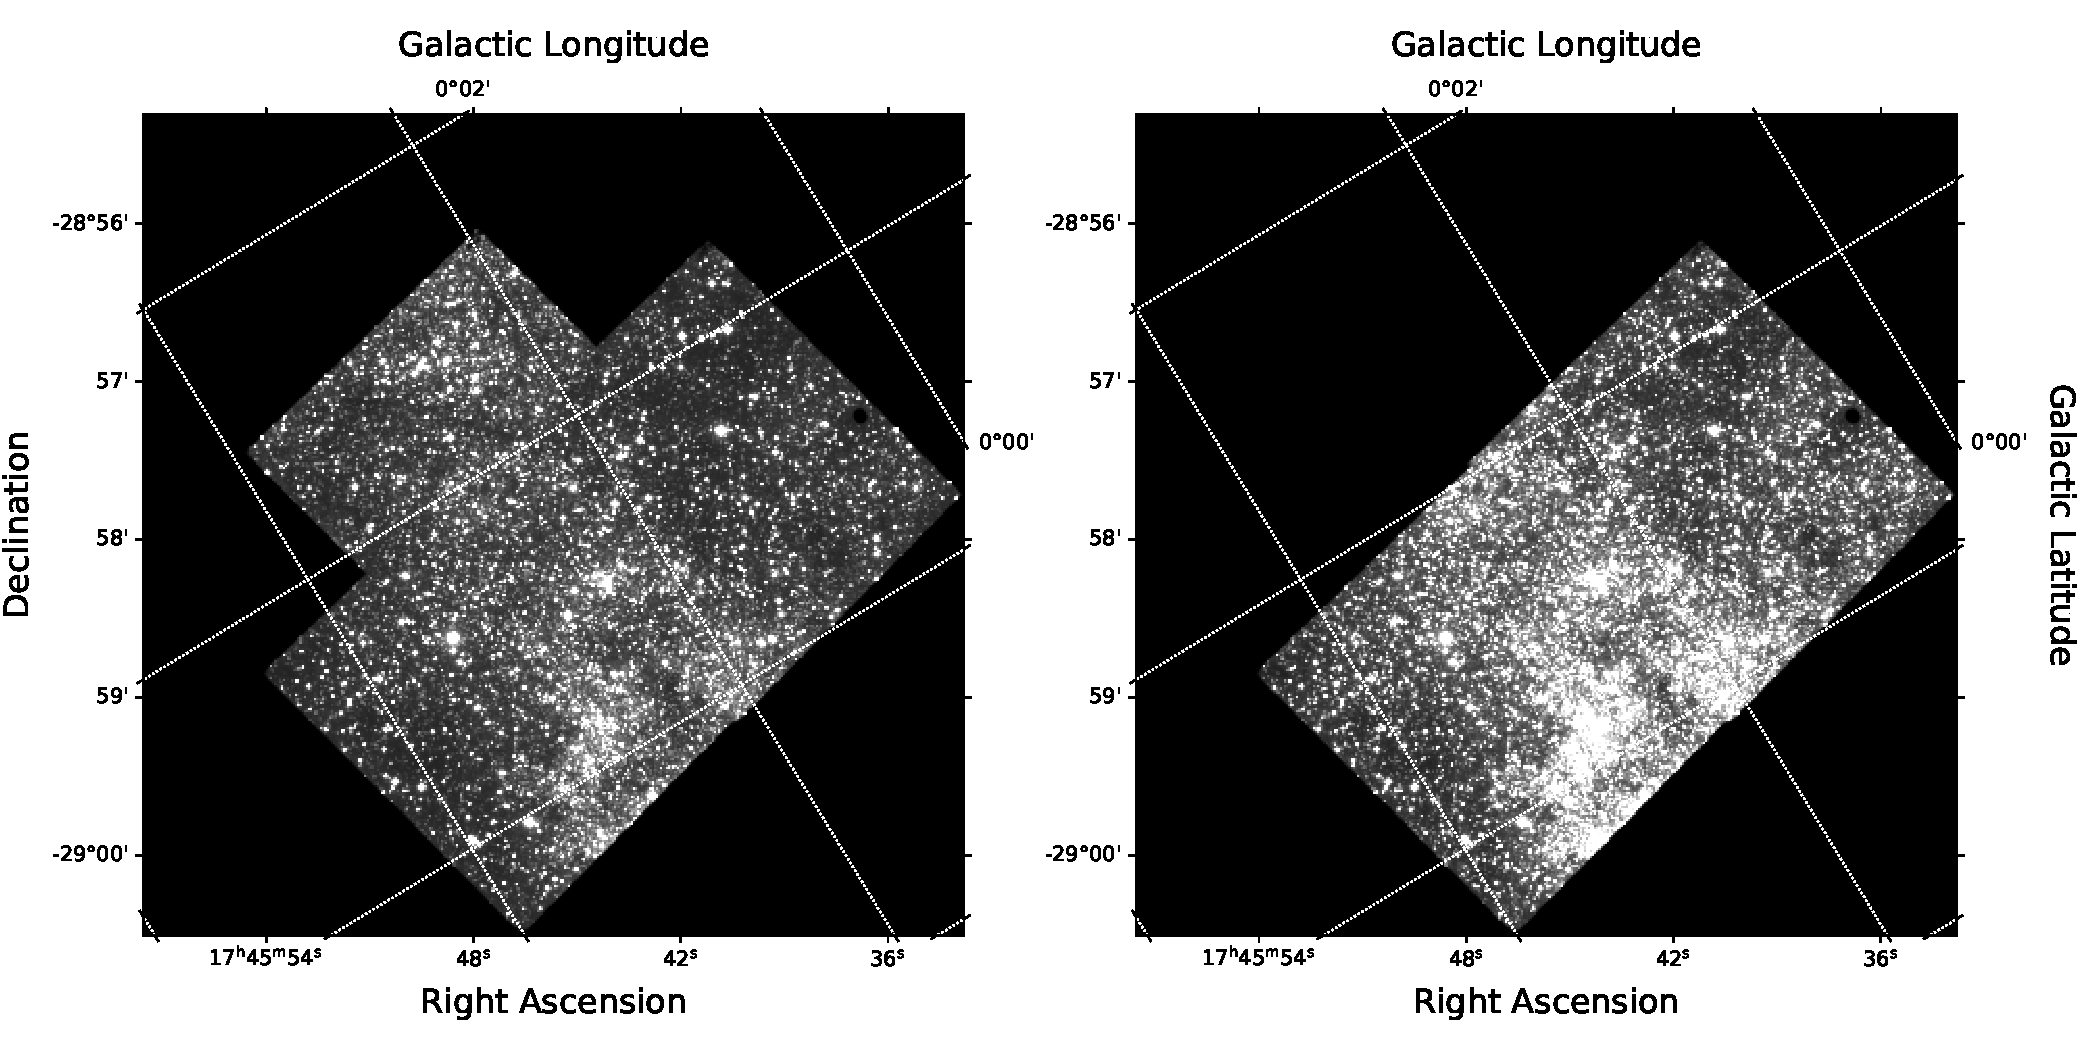
\includegraphics[width=\linewidth]{img/hst_12182_a7_wfc3_ir_f127m_drz.pdf}
  \caption{(\textit{cont.}) Proposal ID 12182 のデータ. 上から順番に MW-NSC-V37, MW-NSC-V41 の領域を示す.}
  \label{fig:12182b}
\end{figure}

\subsection{面輝度ヒストグラム}
バックグラウンド放射強度の推定に使用したヒストグラムを図~\ref{fig:histogram:1} に表示する. 画像の説明はいずれも図~\ref{fig:histogram:arches} と同様である.

\begin{figure}
  \centering
  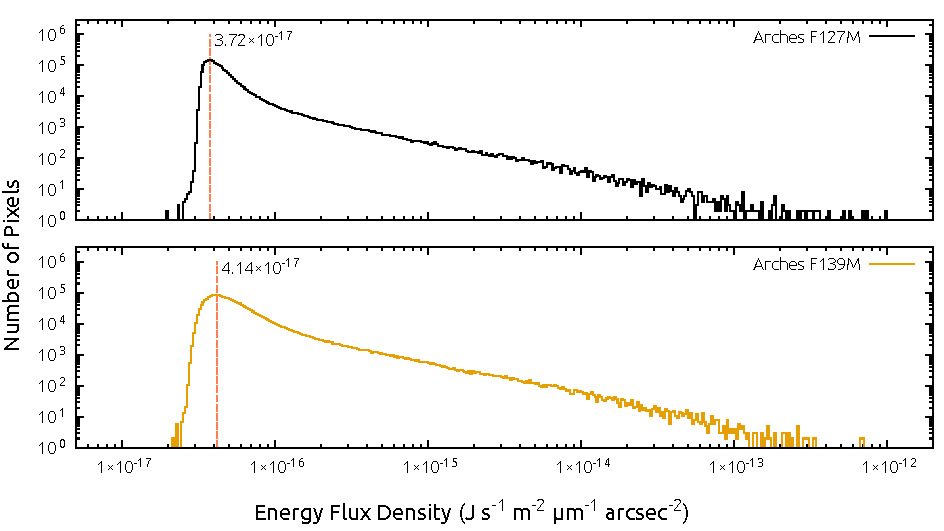
\includegraphics[page=1,width=.9\linewidth]{img/histogram.pdf}
  \includegraphics[page=2,width=.9\linewidth]{img/histogram.pdf}
  \includegraphics[page=3,width=.9\linewidth]{img/histogram.pdf}
  \caption{画像データから作成した面輝度のヒストグラム. 上のパネル (黒) は F127M のデータ, 下のパネル (黄色) は F139M のデータから作成した. ヒストグラムのピーク値をオレンジ色の破線で示した.}
  \label{fig:histogram:1}
\end{figure}

\addtocounter{figure}{-1}
\begin{figure}
  \centering
  \includegraphics[page=4,width=.9\linewidth]{img/histogram.pdf}
  \includegraphics[page=5,width=.9\linewidth]{img/histogram.pdf}
  \includegraphics[page=6,width=.9\linewidth]{img/histogram.pdf}
  \caption{(\textit{cont.}) 画像データから作成した面輝度のヒストグラム.}
  \label{fig:histogram:2}
\end{figure}

\addtocounter{figure}{-1}
\begin{figure}
  \centering
  \includegraphics[page=7,width=.9\linewidth]{img/histogram.pdf}
  \includegraphics[page=8,width=.9\linewidth]{img/histogram.pdf}
  \caption{(\textit{cont.}) 画像データから作成した面輝度のヒストグラム.}
  \label{fig:histogram:3}
\end{figure}

\end{document}
